% !TEX root = ../main.tex

%% !TEX root = ../main.tex

\newcommand{\BP}{\texttt{BP}}
\newcommand{\fp}{$\oplus$}
\newcommand{\fail}{$\times$}
\newcommand{\noSWC}{$\bigcirc$}
\newcommand{\info}{$!$}
\newcommand{\pass}{$\checkmark$}
\newcommand{\na}{}
\newcommand{\tx}[1]{\fontfamily{cmss}\selectfont{\textbf{#1}}}
\newcommand{\ccl}{\cellcolor[HTML]{EFEFEF}}
\newcommand{\rcl}{\rowcolor[HTML]{EFEFEF}}
\newcolumntype{P}[1]{>{\centering\arraybackslash}p{#1}}

\begin{table*}
\centering
\begin{adjustbox}{max height=10cm}
\begin{tabular}{|P{3mm}|P{7mm}|m{105mm}|P{3mm}|P{3mm}|P{3mm}|P{3mm}|P{3mm}|P{3mm}|P{3mm}|}

\multicolumn{3}{c}{\.} &
\headrow{EY Token Review} &
\headrow{Smart Check} &
\headrow{Securify} &
\headrow{MythX (Mythril)} &
\headrow{Contract Guard} &
\headrow{Slither} &
\headrow{Odin} \\ \hline

\rcl\ccl & \ccl & \tx{Vulnerability or best practice} & \multicolumn{7}{c|}{\ccl} \\ \cline{3-3}
\rcl\multirow{-2}{*}{\ccl\tx{ID}} & \multirow{-2}{*}{\ccl\tx{SWC}} & Mitigation or recommendation & \multicolumn{7}{c|}{\multirow{-2}{*}{\ccl\tx{Security tools}}} \\ \hline

\multirow{2}{*}{1} & \multirow{2}{*}{100} & \tx{Function default visibility} & \multirow{2}{*}{\na} & \multirow{2}{*}{\pass} & \multirow{2}{*}{\na} & \multirow{2}{*}{\pass} & \multirow{2}{*}{\pass} & \multirow{2}{*}{\na} & \multirow{2}{*}{\pass} \\ \cline{3-3} & & Specifying function visibility, external, public, internal or private & & & & & & & \\ \hline
\multirow{2}{*}{2} & \multirow{2}{*}{101} & \tx{Integer Overflow and Underflow} & \multirow{2}{*}{\fp} & \multirow{2}{*}{\info} & \multirow{2}{*}{\na} & \multirow{2}{*}{\pass} & \multirow{2}{*}{\pass} & \multirow{2}{*}{\na} & \multirow{2}{*}{\pass} \\ \cline{3-3}
& & Utilizing the SafeMath library to mitigate over/under value assignments & & & & & & & \\ \hline
\multirow{2}{*}{3} & \multirow{2}{*}{102} & \tx{Outdated Compiler Version} & \multirow{2}{*}{\pass} & \multirow{2}{*}{\pass} & \multirow{2}{*}{\pass} & \multirow{2}{*}{\pass} & \multirow{2}{*}{\pass} & \multirow{2}{*}{\pass} & \multirow{2}{*}{\fail} \\ \cline{3-3}
& & Using proper Solidity version to protect against compiler attacks & & & & & & & \\ \hline
\multirow{2}{*}{4} & \multirow{2}{*}{103} & \tx{Floating Pragma} & \multirow{2}{*}{\na} & \multirow{2}{*}{\pass} & \multirow{2}{*}{\pass} & \multirow{2}{*}{\pass} & \multirow{2}{*}{\na} & \multirow{2}{*}{\pass} & \multirow{2}{*}{\pass} \\ \cline{3-3}
& & Locking the pragma to avoid deployments using outdated compiler version & & & & & & & \\ \hline
\multirow{2}{*}{5} & \multirow{2}{*}{104} & \tx{Unchecked Call Return Value} & \multirow{2}{*}{\fp} & \multirow{2}{*}{\na} & \multirow{2}{*}{\pass} & \multirow{2}{*}{\pass} & \multirow{2}{*}{\pass} & \multirow{2}{*}{\fp} & \multirow{2}{*}{\pass} \\ \cline{3-3}
& & Checking call() return value to prevent unexpected behavior in DApps & & & & & & & \\ \hline
\multirow{2}{*}{6} & \multirow{2}{*}{105} & \tx{Unprotected Ether Withdrawal} & \multirow{2}{*}{\na} & \multirow{2}{*}{\info} & \multirow{2}{*}{\na} & \multirow{2}{*}{\pass} & \multirow{2}{*}{\na} & \multirow{2}{*}{\pass} & \multirow{2}{*}{\pass} \\ \cline{3-3}
& & Authorizing only trusted parties to trigger ETH withdrawals & & & & & & & \\ \hline
\multirow{2}{*}{7} & \multirow{2}{*}{106} & \tx{Unprotected SELFDESTRUCT Instruction} & \multirow{2}{*}{\na} & \multirow{2}{*}{\na} & \multirow{2}{*}{\pass} & \multirow{2}{*}{\pass} & \multirow{2}{*}{\na} & \multirow{2}{*}{\pass} & \multirow{2}{*}{\pass} \\ \cline{3-3}
& & Removing self-destruct functionality or approving it by multiple parties & & & & & & & \\ \hline
\multirow{2}{*}{8} & \multirow{2}{*}{107} & \tx{Re-entrancy} & \multirow{2}{*}{\na} & \multirow{2}{*}{\pass} & \multirow{2}{*}{\fp} & \multirow{2}{*}{\fp} & \multirow{2}{*}{\fp} & \multirow{2}{*}{\pass} & \multirow{2}{*}{\pass} \\ \cline{3-3}
& & Using CEI and Mutex to mitigate self-function and cross-function attack & & & & & & & \\ \hline
\multirow{2}{*}{9} & \multirow{2}{*}{108} & \tx{State variable default visibility} & \multirow{2}{*}{\pass} & \multirow{2}{*}{\pass} & \multirow{2}{*}{\pass} & \multirow{2}{*}{\pass} & \multirow{2}{*}{\pass} & \multirow{2}{*}{\na} & \multirow{2}{*}{\pass} \\ \cline{3-3}
& & Specifying visibility of all variables, public, private or internal & & & & & & & \\ \hline
\multirow{2}{*}{10} & \multirow{2}{*}{109} & \tx{Uninitialized Storage Pointer} & \multirow{2}{*}{\pass} & \multirow{2}{*}{\pass} & \multirow{2}{*}{\pass} & \multirow{2}{*}{\pass} & \multirow{2}{*}{\pass} & \multirow{2}{*}{\pass} & \multirow{2}{*}{\pass} \\ \cline{3-3}
& & Initializing variables upon declaration to prevent unexpected storage access & & & & & & & \\ \hline
\multirow{2}{*}{11} & \multirow{2}{*}{110} & \tx{Assert Violation} & \multirow{2}{*}{\na} & \multirow{2}{*}{\pass} & \multirow{2}{*}{\na} & \multirow{2}{*}{\pass} & \multirow{2}{*}{\na} & \multirow{2}{*}{\na} & \multirow{2}{*}{\pass} \\ \cline{3-3}
& & Using require() statement to validate inputs, checking efficiency of the code & & & & & & & \\ \hline
\multirow{2}{*}{12} & \multirow{2}{*}{111} & \tx{Use of Deprecated Solidity Functions} & \multirow{2}{*}{\na} & \multirow{2}{*}{\pass} & \multirow{2}{*}{\na} & \multirow{2}{*}{\pass} & \multirow{2}{*}{\pass} & \multirow{2}{*}{\pass} & \multirow{2}{*}{\pass} \\ \cline{3-3}
& & Using new alternatives functions such as keccak256() instead of sha3() & & & & & & & \\ \hline
\multirow{2}{*}{13} & \multirow{2}{*}{112} & \tx{Delegatecall to untrusted callee} & \multirow{2}{*}{\na} & \multirow{2}{*}{\fp} & \multirow{2}{*}{\fp} & \multirow{2}{*}{\pass} & \multirow{2}{*}{\pass} & \multirow{2}{*}{\pass} & \multirow{2}{*}{\pass} \\ \cline{3-3}
& & Calling into trusted contracts to avoid storage access by malicious contracts & & & & & & & \\ \hline
\multirow{2}{*}{14} & \multirow{2}{*}{113} & \tx{DoS with Failed Call} & \multirow{2}{*}{\pass} & \multirow{2}{*}{\pass} & \multirow{2}{*}{\na} & \multirow{2}{*}{\pass} & \multirow{2}{*}{\pass} & \multirow{2}{*}{\na} & \multirow{2}{*}{\pass} \\ \cline{3-3}
& & Avoid multiple external calls where one error may fail other transactions & & & & & & & \\ \hline
\multirow{2}{*}{15} & \multirow{2}{*}{114} & \tx{Transaction Order Dependence} & \multirow{2}{*}{\fp} & \multirow{2}{*}{\na} & \multirow{2}{*}{\pass} & \multirow{2}{*}{\pass} & \multirow{2}{*}{\na} & \multirow{2}{*}{\na} & \multirow{2}{*}{\pass} \\ \cline{3-3}
& & Preventing race conditions by securing approve() or transferFrom() & & & & & & & \\ \hline
\multirow{2}{*}{16} & \multirow{2}{*}{115} & \tx{Authorization through tx.origin} & \multirow{2}{*}{\pass} & \multirow{2}{*}{\pass} & \multirow{2}{*}{\pass} & \multirow{2}{*}{\pass} & \multirow{2}{*}{\pass} & \multirow{2}{*}{\pass} & \multirow{2}{*}{\pass} \\ \cline{3-3}
& & Using msg.sender to authorize transaction initiator instead of originator & & & & & & & \\ \hline
\multirow{2}{*}{17} & \multirow{2}{*}{116} & \tx{Block values as a proxy for time} & \multirow{2}{*}{\pass} & \multirow{2}{*}{\pass} & \multirow{2}{*}{\pass} & \multirow{2}{*}{\pass} & \multirow{2}{*}{\pass} & \multirow{2}{*}{\na} & \multirow{2}{*}{\pass} \\ \cline{3-3}
& & Not using block.timestamp or block.number to perform functionalities & & & & & & & \\ \hline
\multirow{2}{*}{18} & \multirow{2}{*}{117} & \tx{Signature Malleability} & \multirow{2}{*}{\na} & \multirow{2}{*}{\na} & \multirow{2}{*}{\na} & \multirow{2}{*}{\pass} & \multirow{2}{*}{\na} & \multirow{2}{*}{\na} & \multirow{2}{*}{\pass} \\ \cline{3-3}
& & Not using signed message hash to avoid signatures alteration & & & & & & & \\ \hline
\multirow{2}{*}{19} & \multirow{2}{*}{118} & \tx{Incorrect Constructor Name} & \multirow{2}{*}{\na} & \multirow{2}{*}{\pass} & \multirow{2}{*}{\na} & \multirow{2}{*}{\pass} & \multirow{2}{*}{\na} & \multirow{2}{*}{\na} & \multirow{2}{*}{\pass} \\ \cline{3-3}
& & Using constructor keyword which does not match with contract name & & & & & & & \\ \hline
\multirow{2}{*}{20} & \multirow{2}{*}{119} & \tx{Shadowing State Variables} & \multirow{2}{*}{\na} & \multirow{2}{*}{\na} & \multirow{2}{*}{\pass} & \multirow{2}{*}{\pass} & \multirow{2}{*}{\pass} & \multirow{2}{*}{\pass} & \multirow{2}{*}{\pass} \\ \cline{3-3}
& & Removing any variable ambiguities when inheriting other contracts & & & & & & & \\ \hline
\multirow{2}{*}{21} & \multirow{2}{*}{120} & \tx{Weak Sources of Randomness from Chain Attributes} & \multirow{2}{*}{\pass} & \multirow{2}{*}{\pass} & \multirow{2}{*}{\na} & \multirow{2}{*}{\pass} & \multirow{2}{*}{\pass} & \multirow{2}{*}{\na} & \multirow{2}{*}{\pass} \\ \cline{3-3}
& & Using oracles as source of randomness instead of block.timestamp & & & & & & & \\ \hline
\multirow{2}{*}{22} & \multirow{2}{*}{121} & \tx{Missing Protection against Signature Replay Attacks} & \multirow{2}{*}{\na} & \multirow{2}{*}{\na} & \multirow{2}{*}{\na} & \multirow{2}{*}{\pass} & \multirow{2}{*}{\na} & \multirow{2}{*}{\na} & \multirow{2}{*}{\pass} \\ \cline{3-3}
& & Storing every message hash to perform signature verification & & & & & & & \\ \hline
\multirow{2}{*}{23} & \multirow{2}{*}{122} & \tx{Lack of Proper Signature Verification} & \multirow{2}{*}{\na} & \multirow{2}{*}{\na} & \multirow{2}{*}{\na} & \multirow{2}{*}{\pass} & \multirow{2}{*}{\na} & \multirow{2}{*}{\na} & \multirow{2}{*}{\pass} \\ \cline{3-3}
& & Using alternate verification schemes if allowing off-chain signing & & & & & & & \\ \hline
\multirow{2}{*}{24} & \multirow{2}{*}{123} & \tx{Requirement Violation} & \multirow{2}{*}{\na} & \multirow{2}{*}{\pass} & \multirow{2}{*}{\pass} & \multirow{2}{*}{\pass} & \multirow{2}{*}{\na} & \multirow{2}{*}{\na} & \multirow{2}{*}{\pass} \\ \cline{3-3}
& & Checking the code for allowing only valid external inputs & & & & & & & \\ \hline
\multirow{2}{*}{25} & \multirow{2}{*}{124} & \tx{Write to Arbitrary Storage Location} & \multirow{2}{*}{\na} & \multirow{2}{*}{\pass} & \multirow{2}{*}{\pass} & \multirow{2}{*}{\pass} & \multirow{2}{*}{\na} & \multirow{2}{*}{\na} & \multirow{2}{*}{\pass} \\ \cline{3-3}
& & Controlling write to storage to prevent storage corruption by attackers & & & & & & & \\ \hline
\multirow{2}{*}{26} & \multirow{2}{*}{125} & \tx{Incorrect Inheritance Order} & \multirow{2}{*}{\na} & \multirow{2}{*}{\na} & \multirow{2}{*}{\na} & \multirow{2}{*}{\pass} & \multirow{2}{*}{\na} & \multirow{2}{*}{\na} & \multirow{2}{*}{\pass} \\ \cline{3-3}
& & Inheriting from more general to specific when there are identical functions & & & & & & & \\ \hline
\multirow{2}{*}{27} & \multirow{2}{*}{126} & \tx{Insufficient Gas Griefing} & \multirow{2}{*}{\na} & \multirow{2}{*}{\pass} & \multirow{2}{*}{\na} & \multirow{2}{*}{\na} & \multirow{2}{*}{\na} & \multirow{2}{*}{\na} & \multirow{2}{*}{\pass} \\ \cline{3-3}
& & Allowing trusted forwarders to relay transactions & & & & & & & \\ \hline


\end{tabular}
\end{adjustbox}	
\caption{Auditing results of 7 smart contract analysis tools on \sys. \pass=Passed audit, \fp=False positive, \fail=Failed audit, Empty=Not supported audit by the tool, \info=Informational, \noSWC=Tool specific audit (No SWC registry), BP=Best practice\label{tab:result1}}
\end{table*}

%% !TEX root = ../main.tex

\begin{table*}
\centering
\begin{adjustbox}{max height=10cm}
\begin{tabular}{|P{3mm}|P{7mm}|m{105mm}|P{3mm}|P{3mm}|P{3mm}|P{3mm}|P{3mm}|P{3mm}|P{3mm}|}
	
\multicolumn{3}{c}{\.} &
\headrow{EY Token Review} &
\headrow{Smart Check} &
\headrow{Securify} &
\headrow{MythX (Mythril)} &
\headrow{Contract Guard} &
\headrow{Slither} &
\headrow{Odin} \\ \hline

\rcl\ccl & \ccl & \tx{Vulnerability or best practice} & \multicolumn{7}{c|}{\ccl} \\ \cline{3-3}
\rcl\multirow{-2}{*}{\ccl\tx{ID}} & \multirow{-2}{*}{\ccl\tx{SWC}} & Mitigation or recommendation & \multicolumn{7}{c|}{\multirow{-2}{*}{\ccl\tx{Security tools}}} \\ \hline

\multirow{2}{*}{28} & \multirow{2}{*}{127} & \tx{Arbitrary Jump with Function Type Variable} & \multirow{2}{*}{\na} & \multirow{2}{*}{\pass} & \multirow{2}{*}{\pass} & \multirow{2}{*}{\pass} & \multirow{2}{*}{\na} & \multirow{2}{*}{\pass} & \multirow{2}{*}{\pass} \\ \cline{3-3}
& & Minimizing use of assembly in the code & & & & & & & \\ \hline
\multirow{2}{*}{29} & \multirow{2}{*}{128} & \tx{DoS With Block Gas Limit} & \multirow{2}{*}{\pass} & \multirow{2}{*}{\pass} & \multirow{2}{*}{\pass} & \multirow{2}{*}{\pass} & \multirow{2}{*}{\pass} & \multirow{2}{*}{\pass} & \multirow{2}{*}{\pass} \\ \cline{3-3}
& & Avoiding loops across the code that may consume considerable resources & & & & & & & \\ \hline
\multirow{2}{*}{30} & \multirow{2}{*}{129} & \tx{Typographical Error} & \multirow{2}{*}{\na} & \multirow{2}{*}{\na} & \multirow{2}{*}{\na} & \multirow{2}{*}{\pass} & \multirow{2}{*}{\na} & \multirow{2}{*}{\na} & \multirow{2}{*}{\pass} \\ \cline{3-3}
& & Using SafeMath library or performing checks on any math operation & & & & & & & \\ \hline
\multirow{2}{*}{31} & \multirow{2}{*}{130} & \tx{Right-To-Left-Override control character (U+202E)} & \multirow{2}{*}{\na} & \multirow{2}{*}{\na} & \multirow{2}{*}{\pass} & \multirow{2}{*}{\pass} & \multirow{2}{*}{\pass} & \multirow{2}{*}{\pass} & \multirow{2}{*}{\pass} \\ \cline{3-3}
& & Avoiding U+202E character which forces RTL text rendering & & & & & & & \\ \hline
\multirow{2}{*}{32} & \multirow{2}{*}{131} & \tx{Presence of unused variables} & \multirow{2}{*}{\na} & \multirow{2}{*}{\pass} & \multirow{2}{*}{\pass} & \multirow{2}{*}{\na} & \multirow{2}{*}{\pass} & \multirow{2}{*}{\pass} & \multirow{2}{*}{\fp} \\ \cline{3-3} & & Removing all unused variables to decrease gas consumption & & & & & & & \\ \hline
\multirow{2}{*}{33} & \multirow{2}{*}{132} & \tx{Unexpected Ether balance} & \multirow{2}{*}{\na} & \multirow{2}{*}{\pass} & \multirow{2}{*}{\pass} & \multirow{2}{*}{\na} & \multirow{2}{*}{\pass} & \multirow{2}{*}{\pass} & \multirow{2}{*}{\pass} \\ \cline{3-3} & & Avoiding Ether balance check in the code (\eg this.balance == 0.24 Ether) & & & & & & & \\ \hline
\multirow{2}{*}{34} & \multirow{2}{*}{133} & \tx{Hash Collisions With Variable Length Arguments} & \multirow{2}{*}{\na} & \multirow{2}{*}{\na} & \multirow{2}{*}{\na} & \multirow{2}{*}{\na} & \multirow{2}{*}{\na} & \multirow{2}{*}{\na} & \multirow{2}{*}{\pass} \\ \cline{3-3} & & Using abi.encode() instead of abi.encodePacked() to prevent hash collision & & & & & & & \\ \hline
\multirow{2}{*}{35} & \multirow{2}{*}{134} & \tx{Message call with hardcoded gas amount} & \multirow{2}{*}{\na} & \multirow{2}{*}{\fp} & \multirow{2}{*}{\fp} & \multirow{2}{*}{\pass} & \multirow{2}{*}{\pass} & \multirow{2}{*}{\na} & \multirow{2}{*}{\pass} \\ \cline{3-3} & & Using .call.value()("") which is compatible with EIP1884 & & & & & & & \\ \hline
\multirow{2}{*}{36} & \multirow{2}{*}{135} & \tx{Code With No Effects} & \multirow{2}{*}{\na} & \multirow{2}{*}{\pass} & \multirow{2}{*}{\na} & \multirow{2}{*}{\na} & \multirow{2}{*}{\na} & \multirow{2}{*}{\na} & \multirow{2}{*}{\pass} \\ \cline{3-3} & & Writing unit tests to ensure producing the intended effects by DApps & & & & & & & \\ \hline
\multirow{2}{*}{37} & \multirow{2}{*}{136} & \tx{Unencrypted Private Data On-Chain} & \multirow{2}{*}{\na} & \multirow{2}{*}{\info} & \multirow{2}{*}{\na} & \multirow{2}{*}{\na} & \multirow{2}{*}{\na} & \multirow{2}{*}{\na} & \multirow{2}{*}{\pass} \\ \cline{3-3} & & Storing un-encrypted private data off-chain & & & & & & & \\ \hline
\multirow{2}{*}{38} & \multirow{2}{*}{\noSWC} & \tx{Allowance decreases upon transfer} & \multirow{2}{*}{\pass} & \multirow{2}{*}{\na} & \multirow{2}{*}{\na} & \multirow{2}{*}{\na} & \multirow{2}{*}{\na} & \multirow{2}{*}{\na} & \multirow{2}{*}{\na} \\ \cline{3-3} & & Decreasing allowance in transferFrom() method & & & & & & & \\ \hline
\multirow{2}{*}{39} & \multirow{2}{*}{\noSWC} & \tx{Allowance function returns an accurate value} & \multirow{2}{*}{\pass} & \multirow{2}{*}{\na} & \multirow{2}{*}{\na} & \multirow{2}{*}{\na} & \multirow{2}{*}{\na} & \multirow{2}{*}{\na} & \multirow{2}{*}{\na} \\ \cline{3-3} & & Returning only value from the mapping instead of internal function logic & & & & & & & \\ \hline
\multirow{2}{*}{40} & \multirow{2}{*}{\noSWC} & \tx{It is possible to cancel an existing allowance} & \multirow{2}{*}{\pass} & \multirow{2}{*}{\pass} & \multirow{2}{*}{\na} & \multirow{2}{*}{\na} & \multirow{2}{*}{\na} & \multirow{2}{*}{\na} & \multirow{2}{*}{\na} \\ \cline{3-3} & & Possibility of setting allowance to 0 to revoke previous allowances & & & & & & & \\ \hline
\multirow{2}{*}{41} & \multirow{2}{*}{\noSWC} & \tx{A transfer with an insufficient amount is reverted} & \multirow{2}{*}{\pass} & \multirow{2}{*}{\na} & \multirow{2}{*}{\na} & \multirow{2}{*}{\na} & \multirow{2}{*}{\na} & \multirow{2}{*}{\pass} & \multirow{2}{*}{\na} \\ \cline{3-3} & & Checking balances in transfer() method before updating balances & & & & & & & \\ \hline
\multirow{2}{*}{42} & \multirow{2}{*}{\noSWC} & \tx{Upon sending funds, the sender's balance is updated} & \multirow{2}{*}{\pass} & \multirow{2}{*}{\na} & \multirow{2}{*}{\na} & \multirow{2}{*}{\na} & \multirow{2}{*}{\na} & \multirow{2}{*}{\na} & \multirow{2}{*}{\na} \\ \cline{3-3} & & Updating balances in transfer() or transferFrom() methods & & & & & & & \\ \hline
\multirow{2}{*}{43} & \multirow{2}{*}{\noSWC} & \tx{The Transfer event correctly logged} & \multirow{2}{*}{\pass} & \multirow{2}{*}{\na} & \multirow{2}{*}{\na} & \multirow{2}{*}{\na} & \multirow{2}{*}{\na} & \multirow{2}{*}{\na} & \multirow{2}{*}{\na} \\ \cline{3-3} & & Emitting Transfer event in transfer() or transferFrom() functions & & & & & & & \\ \hline
\multirow{2}{*}{44} & \multirow{2}{*}{\noSWC} & \tx{Transfer an amount that is greater than the allowance} & \multirow{2}{*}{\pass} & \multirow{2}{*}{\na} & \multirow{2}{*}{\na} & \multirow{2}{*}{\na} & \multirow{2}{*}{\na} & \multirow{2}{*}{\na} & \multirow{2}{*}{\na} \\ \cline{3-3} & & Checking balances in transferFrom() method before updating balances & & & & & & & \\ \hline
\multirow{2}{*}{45} & \multirow{2}{*}{\noSWC} & \tx{Risk of short address attack is minimized} & \multirow{2}{*}{\pass} & \multirow{2}{*}{\na} & \multirow{2}{*}{\na} & \multirow{2}{*}{\na} & \multirow{2}{*}{\pass} & \multirow{2}{*}{\na} & \multirow{2}{*}{\na} \\ \cline{3-3} & & Using recent Solidity version to mitigate the attack & & & & & & & \\ \hline
\multirow{2}{*}{46} & \multirow{2}{*}{\noSWC} & \tx{Function names are unique} & \multirow{2}{*}{\pass} & \multirow{2}{*}{\na} & \multirow{2}{*}{\na} & \multirow{2}{*}{\na} & \multirow{2}{*}{\na} & \multirow{2}{*}{\pass} & \multirow{2}{*}{\na} \\ \cline{3-3} & & No function overloading to avoid unexpected behavior & & & & & & & \\ \hline
\multirow{2}{*}{47} & \multirow{2}{*}{\noSWC} & \tx{Using miner controlled variables} & \multirow{2}{*}{\pass} & \multirow{2}{*}{\pass} & \multirow{2}{*}{\pass} & \multirow{2}{*}{\pass} & \multirow{2}{*}{\pass} & \multirow{2}{*}{\pass} & \multirow{2}{*}{\na} \\ \cline{3-3} & & Avoiding block.number, block.timestamp, block.difficulty, now, etc & & & & & & & \\ \hline
\multirow{2}{*}{48} & \multirow{2}{*}{\noSWC} & \tx{Use of return in constructor} & \multirow{2}{*}{\na} & \multirow{2}{*}{\pass} & \multirow{2}{*}{\na} & \multirow{2}{*}{\na} & \multirow{2}{*}{\na} & \multirow{2}{*}{\na} & \multirow{2}{*}{\na} \\ \cline{3-3} & & Not using return in contract's constructor & & & & & & & \\ \hline
\multirow{2}{*}{49} & \multirow{2}{*}{\noSWC} & \tx{Throwing exceptions in transfer() and transferFrom()} & \multirow{2}{*}{\na} & \multirow{2}{*}{\pass} & \multirow{2}{*}{\na} & \multirow{2}{*}{\na} & \multirow{2}{*}{\na} & \multirow{2}{*}{\pass} & \multirow{2}{*}{\na} \\ \cline{3-3} & & Returning true after successful execution or raising exception in failures & & & & & & & \\ \hline
\multirow{2}{*}{50} & \multirow{2}{*}{\noSWC} & \tx{State variables that could be declared constant} & \multirow{2}{*}{\na} & \multirow{2}{*}{\na} & \multirow{2}{*}{\na} & \multirow{2}{*}{\na} & \multirow{2}{*}{\na} & \multirow{2}{*}{\pass} & \multirow{2}{*}{\na} \\ \cline{3-3} & & Adding constant attribute to variables like name, symbol, decimals, etc & & & & & & & \\ \hline
\multirow{2}{*}{51} & \multirow{2}{*}{\noSWC} & \tx{Tautology or contradiction} & \multirow{2}{*}{\na} & \multirow{2}{*}{\na} & \multirow{2}{*}{\na} & \multirow{2}{*}{\na} & \multirow{2}{*}{\na} & \multirow{2}{*}{\pass} & \multirow{2}{*}{\na} \\ \cline{3-3} & & Fixing comparison in the code that are always true or false & & & & & & & \\ \hline
\multirow{2}{*}{52} & \multirow{2}{*}{\noSWC} & \tx{Divide before multiply} & \multirow{2}{*}{\na} & \multirow{2}{*}{\na} & \multirow{2}{*}{\na} & \multirow{2}{*}{\na} & \multirow{2}{*}{\na} & \multirow{2}{*}{\pass} & \multirow{2}{*}{\na} \\ \cline{3-3} & & Ordering multiplication prior division to avoid integer truncation & & & & & & & \\ \hline
\multirow{2}{*}{53} & \multirow{2}{*}{\noSWC} & \tx{Unchecked Send} & \multirow{2}{*}{\na} & \multirow{2}{*}{\na} & \multirow{2}{*}{\na} & \multirow{2}{*}{\na} & \multirow{2}{*}{\na} & \multirow{2}{*}{\pass} & \multirow{2}{*}{\na} \\ \cline{3-3} & & Ensuring that the return value of send() is always checked & & & & & & & \\ \hline
\multirow{2}{*}{54} & \multirow{2}{*}{\BP} & \tx{Too many digits} & \multirow{2}{*}{\na} & \multirow{2}{*}{\na} & \multirow{2}{*}{\na} & \multirow{2}{*}{\na} & \multirow{2}{*}{\na} & \multirow{2}{*}{\pass} & \multirow{2}{*}{\na} \\ \cline{3-3} & & Using scientific notation to make the code readable and simpler to debug & & & & & & & \\ \hline

\end{tabular}
\end{adjustbox}	
\caption{Continuation of Table~\ref{tab:result1}.\label{tab:result2}}
\end{table*}

%% !TEX root = ../main.tex

\begin{table*}
\centering
\begin{adjustbox}{max height=10cm}
\begin{tabular}{|P{3mm}|P{7mm}|m{95mm}|P{7mm}|P{7mm}|P{7mm}|P{7mm}|P{7mm}|P{7mm}|P{7mm}|}

\multicolumn{3}{c}{\.} &
\headrow{EY Token Review} &
\headrow{Smart Check} &
\headrow{Securify} &
\headrow{MythX (Mythril)} &
\headrow{Contract Guard} &
\headrow{Slither} &
\headrow{Odin} \\ \hline

\rcl\ccl & \ccl & \tx{Vulnerability or best practice} & \multicolumn{7}{c|}{\ccl} \\ \cline{3-3}
\rcl\multirow{-2}{*}{\ccl\tx{ID}} & \multirow{-2}{*}{\ccl\tx{SWC}} & Mitigation or recommendation & \multicolumn{7}{c|}{\multirow{-2}{*}{\ccl\tx{Security tools}}} \\ \hline

\multirow{2}{*}{55} & \multirow{2}{*}{\BP} & \tx{The decreaseAllowance definition follows the standard} & \multirow{2}{*}{\pass} & \multirow{2}{*}{\na} & \multirow{2}{*}{\na} & \multirow{2}{*}{\na} & \multirow{2}{*}{\na} & \multirow{2}{*}{\na} & \multirow{2}{*}{\na} \\ \cline{3-3} & & Defining decreaseAllowance input and output variables as standard & & & & & & & \\ \hline
\multirow{2}{*}{56} & \multirow{2}{*}{\BP} & \tx{The increaseAllowance definition follows the standard} & \multirow{2}{*}{\pass} & \multirow{2}{*}{\na} & \multirow{2}{*}{\na} & \multirow{2}{*}{\na} & \multirow{2}{*}{\na} & \multirow{2}{*}{\na} & \multirow{2}{*}{\na} \\ \cline{3-3} & & Defining increaseAllowance input and output variables as standard & & & & & & & \\ \hline
\multirow{2}{*}{57} & \multirow{2}{*}{\BP} & \tx{Minimize attack surface} & \multirow{2}{*}{\pass} & \multirow{2}{*}{\pass} & \multirow{2}{*}{\pass} & \multirow{2}{*}{\na} & \multirow{2}{*}{\na} & \multirow{2}{*}{\na} & \multirow{2}{*}{\na} \\ \cline{3-3} & & Checking whether all the external functions are necessary or not & & & & & & & \\ \hline
\multirow{2}{*}{58} & \multirow{2}{*}{\BP} & \tx{Transfer to the burn address is reverted} & \multirow{2}{*}{\pass} & \multirow{2}{*}{\na} & \multirow{2}{*}{\na} & \multirow{2}{*}{\na} & \multirow{2}{*}{\na} & \multirow{2}{*}{\na} & \multirow{2}{*}{\na} \\ \cline{3-3} & & Reverting transfer to 0x0 due to risk of total supply reduction & & & & & & & \\ \hline
\multirow{2}{*}{59} & \multirow{2}{*}{\BP} & \tx{Source code is decentralized} & \multirow{2}{*}{\pass} & \multirow{2}{*}{\pass} & \multirow{2}{*}{\na} & \multirow{2}{*}{\na} & \multirow{2}{*}{\na} & \multirow{2}{*}{\na} & \multirow{2}{*}{\na} \\ \cline{3-3} & & Not using hard-coded addresses in the code & & & & & & & \\ \hline
\multirow{2}{*}{60} & \multirow{2}{*}{\BP} & \tx{Funds can be held only by user-controlled wallets} & \multirow{2}{*}{\info} & \multirow{2}{*}{\na} & \multirow{2}{*}{\na} & \multirow{2}{*}{\na} & \multirow{2}{*}{\na} & \multirow{2}{*}{\na} & \multirow{2}{*}{\na} \\ \cline{3-3} & & Transferring tokens to users to avoid creating a secondary market & & & & & & & \\ \hline
\multirow{2}{*}{61} & \multirow{2}{*}{\BP} & \tx{Code logic is simple to understand} & \multirow{2}{*}{\pass} & \multirow{2}{*}{\pass} & \multirow{2}{*}{\na} & \multirow{2}{*}{\na} & \multirow{2}{*}{\na} & \multirow{2}{*}{\na} & \multirow{2}{*}{\na} \\ \cline{3-3} & & Avoiding code nesting which makes the code less intuitive & & & & & & & \\ \hline
\multirow{2}{*}{62} & \multirow{2}{*}{\BP} & \tx{All functions are documented} & \multirow{2}{*}{\pass} & \multirow{2}{*}{\na} & \multirow{2}{*}{\na} &\multirow{2}{*}{\na} & \multirow{2}{*}{\na} & \multirow{2}{*}{\na} & \multirow{2}{*}{\na} \\ \cline{3-3} & & Using NatSpec format to explain expected behavior of functions & & & & & & & \\ \hline
\multirow{2}{*}{63} & \multirow{2}{*}{\BP} & \tx{The Approval event is correctly logged} & \multirow{2}{*}{\pass} & \multirow{2}{*}{\na} & \multirow{2}{*}{\na} & \multirow{2}{*}{\na} & \multirow{2}{*}{\na} & \multirow{2}{*}{\na} & \multirow{2}{*}{\na} \\ \cline{3-3} & & Emitting Approval event in the approve() method & & & & & & & \\ \hline
\multirow{2}{*}{64} & \multirow{2}{*}{\BP} & \tx{Acceptable gas cost of the approve() function} & \multirow{2}{*}{\info} & \multirow{2}{*}{\na} & \multirow{2}{*}{\na} & \multirow{2}{*}{\na} & \multirow{2}{*}{\na} & \multirow{2}{*}{\na} & \multirow{2}{*}{\na} \\ \cline{3-3} & & Checking for maximum 50000 gas cost when executing the approve() & & & & & & & \\ \hline
\multirow{2}{*}{65} & \multirow{2}{*}{\BP} & \tx{Acceptable gas cost of the transfer() function} & \multirow{2}{*}{\info} & \multirow{2}{*}{\na} & \multirow{2}{*}{\na} & \multirow{2}{*}{\na} & \multirow{2}{*}{\na} & \multirow{2}{*}{\na} & \multirow{2}{*}{\na} \\ \cline{3-3} & & Checking for maximum 60000 gas cost when executing the transfer() & & & & & & & \\ \hline
\multirow{2}{*}{66} & \multirow{2}{*}{\BP} & \tx{Emitting event when state changes} & \multirow{2}{*}{\pass} & \multirow{2}{*}{\na} & \multirow{2}{*}{\na} & \multirow{2}{*}{\na} & \multirow{2}{*}{\na} & \multirow{2}{*}{\na} & \multirow{2}{*}{\na} \\ \cline{3-3} & & Emitting Change event when changing state variable values & & & & & & & \\ \hline
\multirow{2}{*}{67} & \multirow{2}{*}{\BP} & \tx{Use of unindexed arguments} & \multirow{2}{*}{\na} & \multirow{2}{*}{\pass} & \multirow{2}{*}{\na} & \multirow{2}{*}{\na} & \multirow{2}{*}{\pass} & \multirow{2}{*}{\pass} & \multirow{2}{*}{\na} \\ \cline{3-3} & & Using indexed arguments to facilitate external tools log searching & & & & & & & \\ \hline
\multirow{2}{*}{68} & \multirow{2}{*}{\BP} & \tx{\erc compliance} & \multirow{2}{*}{\pass} & \multirow{2}{*}{\pass} & \multirow{2}{*}{\pass} & \multirow{2}{*}{\na} & \multirow{2}{*}{\pass} & \multirow{2}{*}{\pass} & \multirow{2}{*}{\na} \\ \cline{3-3} & & Implementing all 6 functions and 2 events as specified in EIP-20 & & & & & & & \\ \hline
\multirow{2}{*}{69} & \multirow{2}{*}{\BP} & \tx{Conformance to naming conventions} & \multirow{2}{*}{\na} & \multirow{2}{*}{\na} & \multirow{2}{*}{\na} & \multirow{2}{*}{\na} & \multirow{2}{*}{\na} & \multirow{2}{*}{\pass} & \multirow{2}{*}{\na} \\ \cline{3-3} & & Following the Solidity naming convention to avoid confusion & & & & & & & \\ \hline
\multirow{2}{*}{70} & \multirow{2}{*}{\BP} & \tx{Token decimal} & \multirow{2}{*}{\pass} & \multirow{2}{*}{\na} & \multirow{2}{*}{\na} & \multirow{2}{*}{\na} & \multirow{2}{*}{\na} & \multirow{2}{*}{\na} & \multirow{2}{*}{\na} \\ \cline{3-3} & & Declaring token decimal for external apps when displaying balances & & & & & & & \\ \hline
\multirow{2}{*}{71} & \multirow{2}{*}{\BP} & \tx{Locked money (Freezing ETH)} & \multirow{2}{*}{\na} &\multirow{2}{*}{\pass} & \multirow{2}{*}{\na} & \multirow{2}{*}{\na} & \multirow{2}{*}{\pass} & \multirow{2}{*}{\pass} & \multirow{2}{*}{\na} \\ \cline{3-3} & & Implementing withdraw/reject functions to avoid ETH lost & & & & & & & \\ \hline
\multirow{2}{*}{72} & \multirow{2}{*}{\BP} & \tx{Malicious libraries} & \multirow{2}{*}{\na} & \multirow{2}{*}{\pass} & \multirow{2}{*}{\na} & \multirow{2}{*}{\na} & \multirow{2}{*}{\na} & \multirow{2}{*}{\na} & \multirow{2}{*}{\na} \\ \cline{3-3} & & Not using modifiable third-party libraries & & & & & & & \\ \hline
\multirow{2}{*}{73} & \multirow{2}{*}{\BP} & \tx{Payable fallback function} & \multirow{2}{*}{\na} & \multirow{2}{*}{\pass} & \multirow{2}{*}{\na} & \multirow{2}{*}{\na} & \multirow{2}{*}{\pass} & \multirow{2}{*}{\na} & \multirow{2}{*}{\na} \\ \cline{3-3} & & Adding either fallback() or receive() function to receive ETH & & & & & & & \\ \hline
F\multirow{2}{*}{74} & \multirow{2}{*}{\BP} & \tx{Prefer external to public visibility level} & \multirow{2}{*}{\na} & \multirow{2}{*}{\pass} & \multirow{2}{*}{\na} & \multirow{2}{*}{\na} & \multirow{2}{*}{\na} & \multirow{2}{*}{\pass} & \multirow{2}{*}{\na} \\ \cline{3-3} & & Improving the performance by replacing public with external & & & & & & & \\ \hline
\multirow{2}{*}{75} & \multirow{2}{*}{\BP} & \tx{Token name} & \multirow{2}{*}{\pass} & \multirow{2}{*}{\na} & \multirow{2}{*}{\na} & \multirow{2}{*}{\na} & \multirow{2}{*}{\na} & \multirow{2}{*}{\na} & \multirow{2}{*}{\na} \\ \cline{3-3} & & Adding a token name variable for external apps & & & & & & & \\ \hline
\multirow{2}{*}{76} & \multirow{2}{*}{\BP} & \tx{Error information in revert condition} & \multirow{2}{*}{\na} & \multirow{2}{*}{\na} & \multirow{2}{*}{\na} & \multirow{2}{*}{\na} & \multirow{2}{*}{\pass} & \multirow{2}{*}{\na} & \multirow{2}{*}{\na} \\ \cline{3-3} & & Adding error description in require()/revert() to clarify the reason & & & & & & & \\ \hline
\multirow{2}{*}{77} & \multirow{2}{*}{\BP} & \tx{Complex Fallback} & \multirow{2}{*}{\na} & \multirow{2}{*}{\na} & \multirow{2}{*}{\na} & \multirow{2}{*}{\na} & \multirow{2}{*}{\pass} & \multirow{2}{*}{\na} & \multirow{2}{*}{\na} \\ \cline{3-3} & & Logging operations in the fallback() to avoid complex operations & & & & & & & \\ \hline
\multirow{2}{*}{78} & \multirow{2}{*}{\BP} & \tx{Function Order} & \multirow{2}{*}{\na} & \multirow{2}{*}{\na} & \multirow{2}{*}{\na} & \multirow{2}{*}{\na} & \multirow{2}{*}{\pass} & \multirow{2}{*}{\na} & \multirow{2}{*}{\na} \\ \cline{3-3} & & Following fallback, external, public, internal and private order & & & & & & & \\ \hline
\multirow{2}{*}{79} & \multirow{2}{*}{\BP} & \tx{Visibility Modifier Order} & \multirow{2}{*}{\na} & \multirow{2}{*}{\na} & \multirow{2}{*}{\na} & \multirow{2}{*}{\na} & \multirow{2}{*}{\na} & \multirow{2}{*}{\pass} & \multirow{2}{*}{\na} \\ \cline{3-3} & & Specifying visibility first and before modifiers in functions & & & & & & & \\ \hline
\multirow{2}{*}{80} & \multirow{2}{*}{\BP} & \tx{Non-initialized return value} & \multirow{2}{*}{\na} & \multirow{2}{*}{\pass} & \multirow{2}{*}{\na} & \multirow{2}{*}{\na} & \multirow{2}{*}{\pass} & \multirow{2}{*}{\na} & \multirow{2}{*}{\na} \\ \cline{3-3} & & Not specifying return for functions without output & & & & & & & \\ \hline
\multirow{2}{*}{81} & \multirow{2}{*}{\BP} & \tx{Token symbol} & \multirow{2}{*}{\pass} & \multirow{2}{*}{\na} & \multirow{2}{*}{\na} & \multirow{2}{*}{\na} & \multirow{2}{*}{\na} & \multirow{2}{*}{\na} & \multirow{2}{*}{\na} \\ \cline{3-3} & & Adding token symbol variable for usage of external apps & & & & & & & \\ \hline
\multirow{2}{*}{82} & \multirow{2}{*}{\BP} & \tx{Allowance spending is possible} & \multirow{2}{*}{\pass} & \multirow{2}{*}{\na} & \multirow{2}{*}{\na} & \multirow{2}{*}{\na} & \multirow{2}{*}{\na} & \multirow{2}{*}{\na} & \multirow{2}{*}{\na} \\ \cline{3-3} & & Ability of token transfer by transferFrom() to transfer tokens on behalf of another usercalc & & & & & & & \\ \hline

\hline
\rcl
\multicolumn{3}{|c|}{\ccl\tx{\begin{tabular}[c]{@{}c@{}}\prct success rate in performed audits by considering\\ 'False Positives' and 'Informational' checks as 'Passed' \\ (More details in section~\ref{section:tools}) \end{tabular}}}  & 100\% & 100\% & 100\% & 100\% & 100\% & 100\% & 97\% \\ \hline


\end{tabular}
\end{adjustbox}	
\caption{Continuation of Table~\ref{tab:result2}.\label{tab:result3}}
\end{table*}


\section{Full set of vulnerabilities and auditing results}\label{subsec:audits}
The full results of 7 auditing tools run on the Solidity implementation of \sys are provided. We do not describe each vulnerability or best practice at the same level of detail as the ones we highlight in sections~\ref{sec:vul} and~\ref{sec:bp}, however we will include a simple statement describing the issue and the mitigation. We emphasize that categorizing the tests, checking that a specific test is the same across all the tools, validating that a false positive is not an actual vulnerability, and standardizing the cross-references to the SWC registry are all our own contribution. The quality of a result returned by an actual tools varies and does not always lend itself to easy categorization in our charts. 

\begin{figure*}[t!]
	\centering
	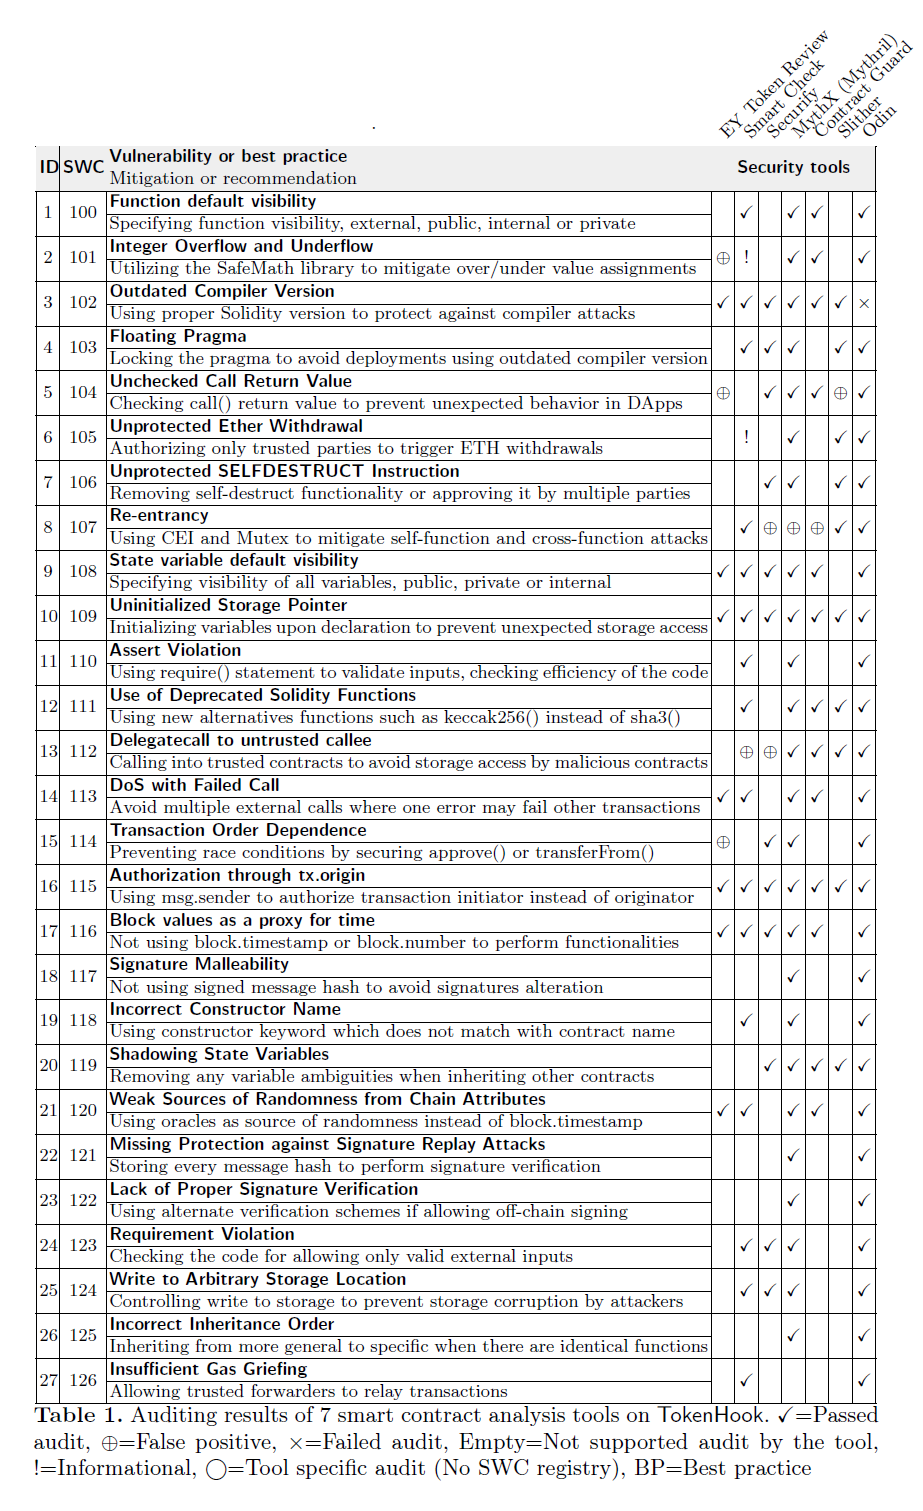
\includegraphics[width=0.9\textwidth]{figures/table1.png}
\end{figure*}

\begin{figure*}[t!]
	\centering
	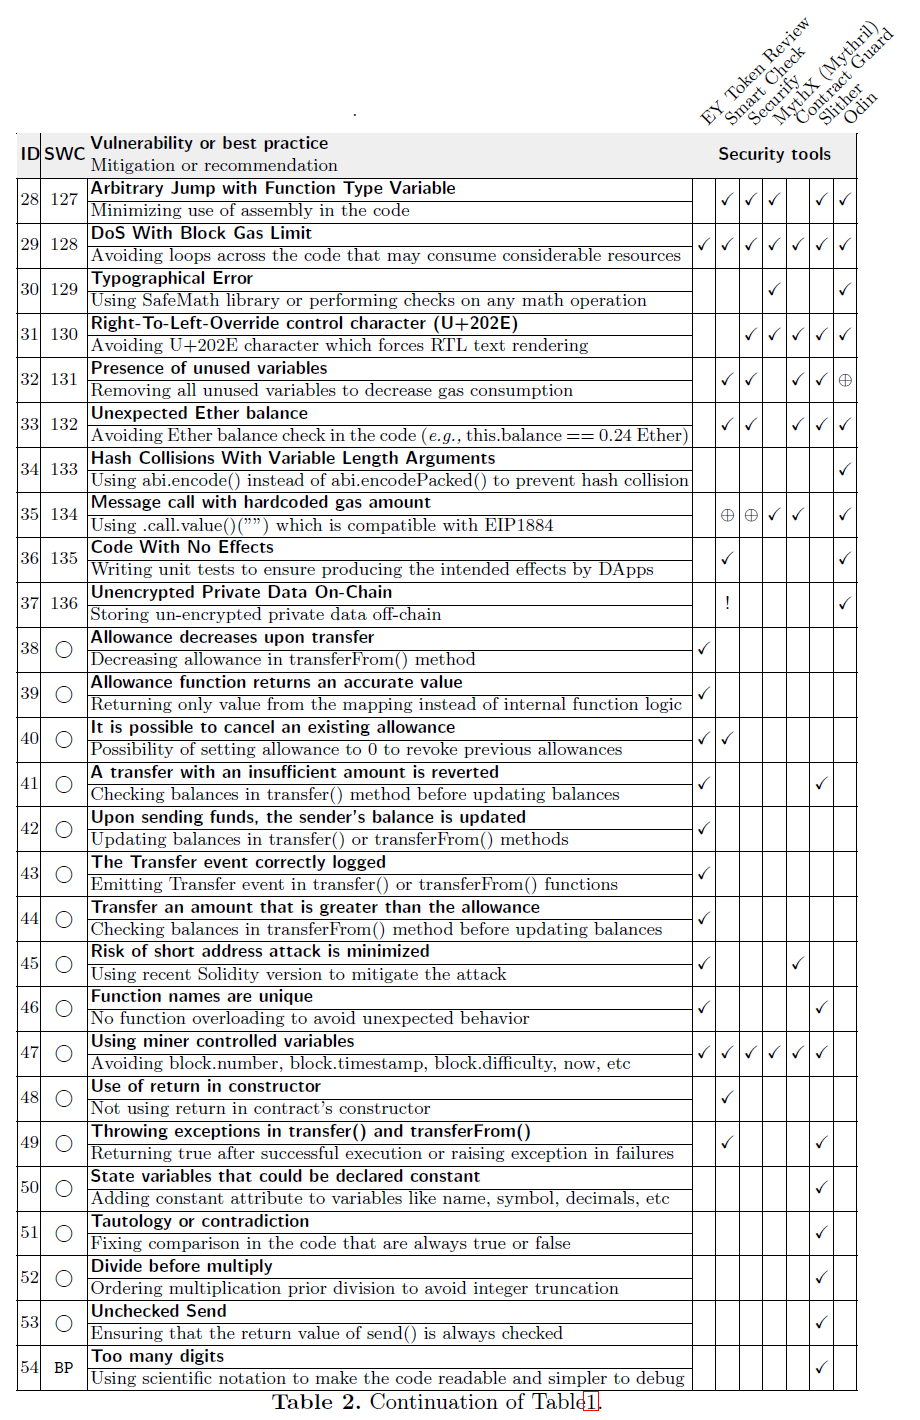
\includegraphics[width=0.9\textwidth]{figures/table2.png}
\end{figure*}

\begin{figure*}[t!]
	\centering
	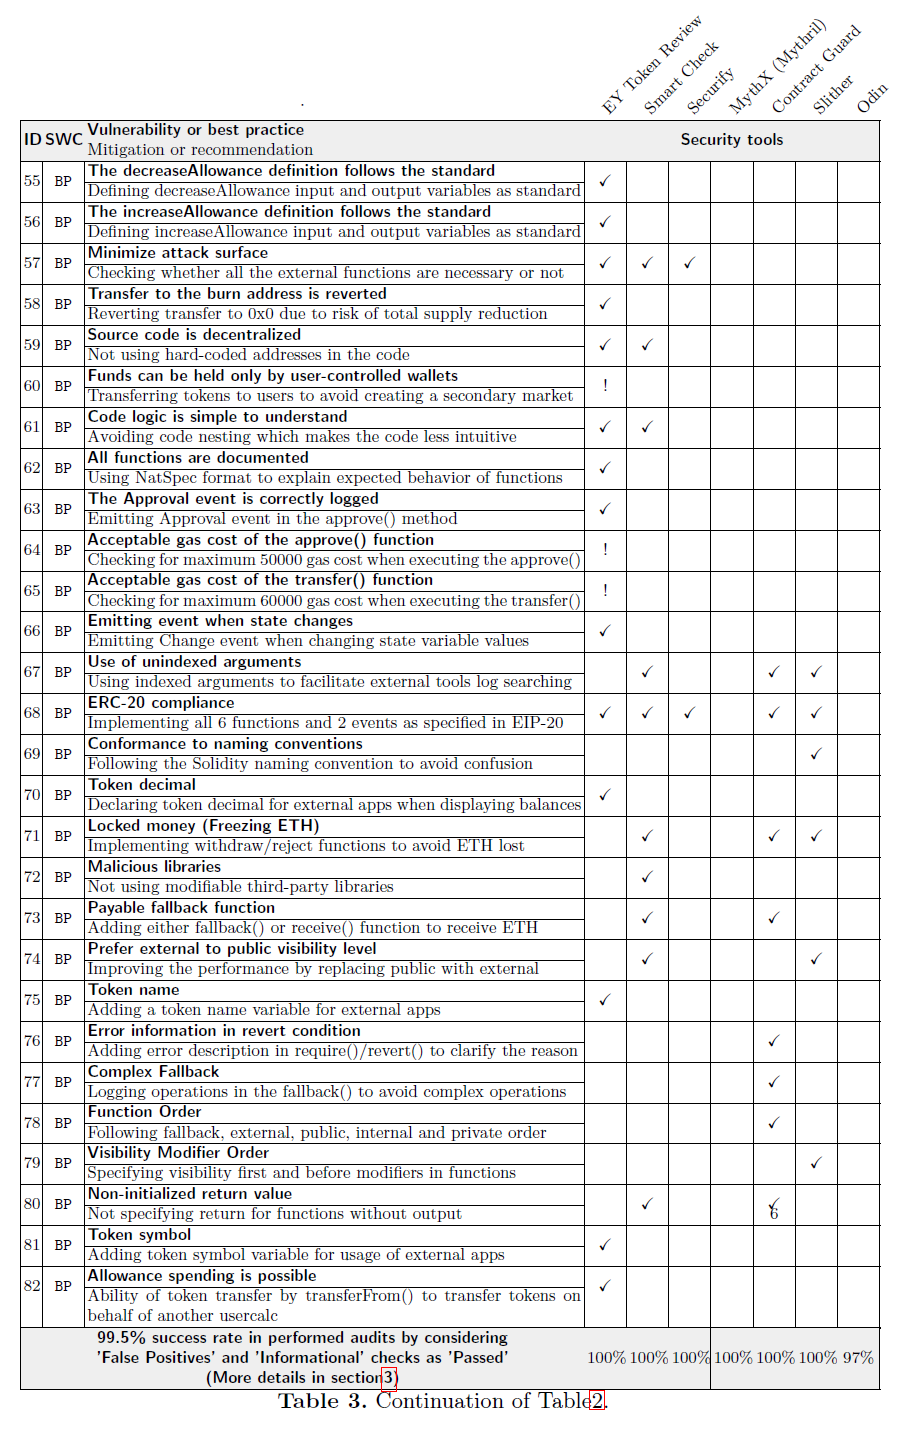
\includegraphics[width=0.9\textwidth]{figures/table3.png}
\end{figure*}

